\let\negmedspace\undefined
\let\negthickspace\undefined
\documentclass[journal]{IEEEtran}
\usepackage[a5paper, margin=10mm, onecolumn]{geometry}
%\usepackage{lmodern} % Ensure lmodern is loaded for pdflatex
\usepackage{tfrupee} % Include tfrupee package

\setlength{\headheight}{1cm} % Set the height of the header box
\setlength{\headsep}{0mm}     % Set the distance between the header box and the top of the text
\usepackage{gvv-book}
\usepackage{gvv}
\usepackage{cite}
\usepackage{amsmath,amssymb,amsfonts,amsthm}
\usepackage{algorithmic}
\usepackage{graphicx}
\usepackage{textcomp}
\usepackage{xcolor}
\usepackage{txfonts}
\usepackage{listings}
\usepackage{enumitem}
\usepackage{mathtools}
\usepackage{gensymb}
\usepackage{comment}
\usepackage[breaklinks=true]{hyperref}
\usepackage{tkz-euclide} 
\usepackage{listings}
\def\inputGnumericTable{}                                 
\usepackage[latin1]{inputenc}                                
\usepackage{color}                                            
\usepackage{array}                                            
\usepackage{longtable}                                       
\usepackage{calc}                                             
\usepackage{multirow}                                         
\usepackage{hhline}                                           
\usepackage{ifthen}                                           
\usepackage{lscape}
\begin{document}

\bibliographystyle{IEEEtran}
\vspace{3cm}

\title{11.16.2.2.3}
\author{EE24BTECH11027 - satwikagv}
% \maketitle
% \newpage
% \bigskip
{\let\newpage\relax\maketitle}

\renewcommand{\thefigure}{\theenumi}
\renewcommand{\thetable}{\theenumi}
\setlength{\intextsep}{10pt} % Space between text and floats


\numberwithin{equation}{enumi}
\numberwithin{figure}{enumi}
\renewcommand{\thetable}{\theenumi}
\textbf{Question:}\\
Find the PMF of the event - a multiple of 3, when a die is thrown.\\ 
\textbf{Solution:}\\
\textbf{Theoretical solution:}\\
We define a random variable $X$ as $X$ : outcome of the die when thrown, is a multiple of 3.\\
The possible outcomes of a die when thrown are \cbrak{1,2,3,4,5,6}. From these, the multiples of 3 are 3 and 6.\\
Therefore $X$ can take the values of 3 and 6. So, the probability space for $X$ is \cbrak{3,6} and the outcomes are equally likely.\\
%Let say the probability that $X=3$ is $p$ and $X=6$ is $1-p$.\\
So, the $PMF$ of $X$ is 
\begin{align}
    P\brak{X=x}= \begin{cases}
        \frac{1}{2}, & x=3,6\\
        0, & \text{otherwise}
    \end{cases}
\end{align}
\textbf{Simulation:}\\
We can simulate this event by rolling a die multiple times and keeping only the outcomes which are multiples of 3.We count the number of 3 and 6 and normalize them.\\
The more number of rolls gives the more accuracy in simulation.\\
The below graph shows the comparison between both the simulation and theoretical probabilities.\\
\textbf{Plot:}\\
\begin{figure}[h!]
   \centering
   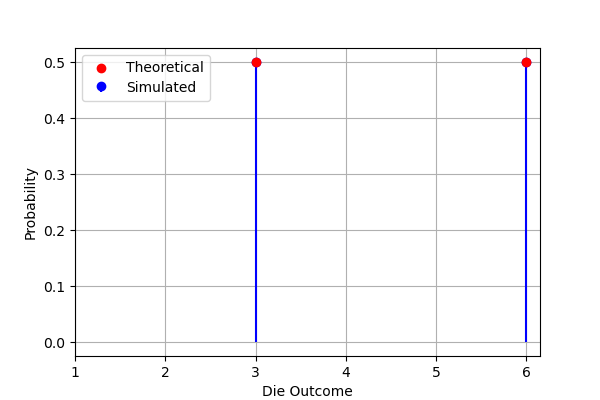
\includegraphics[width=1\columnwidth]{figs/fig.png}
   \caption{PMF of the event a multiple of 3 when a die is thrown}
\end{figure}

\end{document}
